\section{Method}

The method reconstructs a prompt-dominant LLM prototype into a traceable LLM-agent architecture. The language model remains responsible for language composition, and source selection, entity routing, claim eligibility, answer structure, trace logging, and validation are represented as explicit artifacts.

\subsection{Architecture Overview}

\vspace{0.35\baselineskip}

\begin{figure}[H]
    \centering
    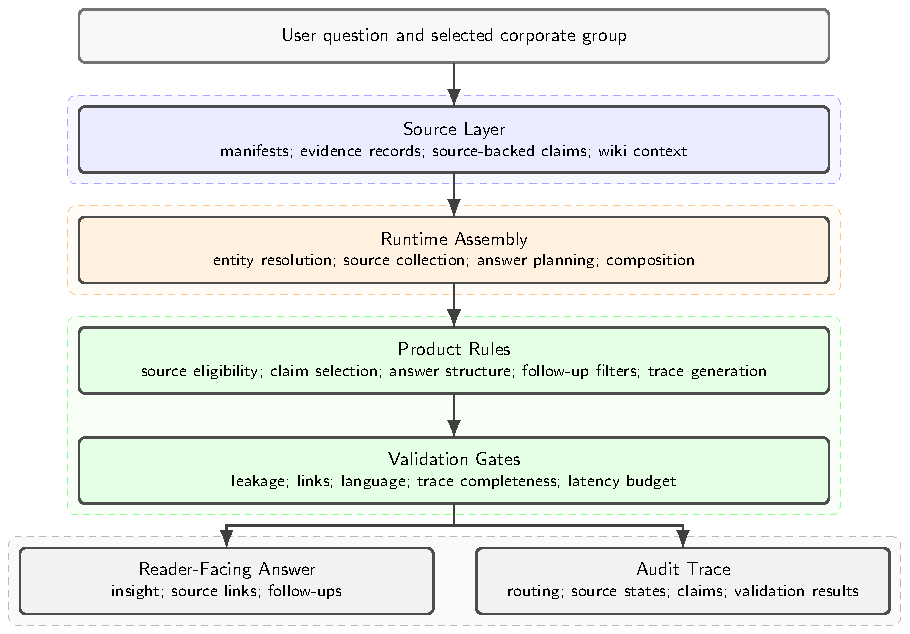
\includegraphics[width=0.95\linewidth,height=0.50\textheight,keepaspectratio]{figures/harness_architecture.pdf}
    \caption{Traceable LLM-agent harness. The architecture separates source authority, runtime assembly, product rules, validation gates, and two outputs: a reader-facing answer and an audit trace.}
    \label{fig:harness-architecture}
\end{figure}

The architecture in \Cref{fig:harness-architecture} starts from a user question and a selected Korean corporate group. The selected entity resolves aliases, market identifiers, filing identifiers, and source namespaces. The runtime returns a reader-facing answer and an audit trace. The trace records routing, source collection, claim selection, answer assembly, and validation, while the control layer manages source eligibility, answer structure, validation, and trace generation.

\subsection{Source-to-Claim Pipeline}

The system first registers raw materials as source manifests. A manifest records the corporate-group scope, company scope, source title, issuer, source category, public URL or filing identifier, local path when available, checksum, rights policy, selection rule, and runtime use policy. Manifest registration prevents the knowledge base from becoming an unbounded document folder.

Documents that pass the source gate are extracted or manually reviewed. Evidence records store file hashes, extracted-text hashes, and evidence locations such as page or line references when available. The system then produces claim candidates. A candidate becomes runtime-eligible only when it is promoted into a source-backed claim: an atomic statement linked to a source manifest, evidence record, claim type, company scope, use policy, and verification state. The claim layer is a key design boundary in our architecture. The model may use source-backed claims as bounded context; related documents require claim promotion before they authorize factual statements.

\subsection{Knowledge Layer and Product Rules}

Following the LLM Wiki pattern, the system maintains markdown knowledge pages that sit between raw source documents and runtime answers \citep{karpathy2026llmwiki}. In our implementation, the maintained knowledge layer is compiled from reviewed artifacts and functions as a context layer. The maintained knowledge layer gives humans and LLMs concise context; source manifests and source-backed claims remain authoritative.

The reconstruction also moves product rules out of the prompt. Entity routing, source eligibility, runtime source state, claim selection, answer-section planning, follow-up filtering, output validation, internal-trace separation, and stage-gate checks are implemented as code, manifests, schemas, and validators. The prompt is kept short and policy-oriented. The prompt-to-code migration is intended to reduce the burden on the model and make diagnostic boundaries easier to locate; direct measurement of prompt-complexity reduction is left to later work.

\subsection{Runtime Answer Assembly}

At runtime, the control layer resolves the selected corporate group and company, collects filing, market, news, wiki, and claim context, builds an answer plan, generates the visible response, validates the output contract, and records the trace. The process trace records tool and source states such as live, local, fallback, fixture, or error. The answer-assembly trace records routing, source collection, claim selection, answer planning, and validation-check results.

The visible answer follows an insight-first contract. It must begin with a reader-facing interpretation, then provide supporting signals, risks or contradictions, source links, and follow-up questions. Follow-up questions are treated as part of the output contract: the reference implementation generates them with a deterministic topic-conditioned builder, and validation checks that enough customer-facing follow-ups are present and free of generic or internal-review wording. Internal artifacts such as claim identifiers, raw trace JSON, and API status labels are reserved for the internal review interface.

\subsection{Reference Implementation}
\label{sec:implementation-details}

The reference implementation is a TypeScript application with JavaScript Object Notation (JSON) source, claim, scenario, and evaluation artifacts. The public release reference is recorded as a placeholder repository citation and should be replaced with the final GitHub URL and submission commit hash before submission \citep{ahnkim2026advisorrepo}. The baseline reported in the paper uses a deterministic, schema-checked composer for fixed validation scenarios and runtime-interface tests. The composer is a rule-based template engine that fills validated answer sections from selected source-backed claims using no generative model call. This baseline fixes the system contract and separates validation of the control layer from model sampling effects.

The architecture treats composition as a replaceable boundary. Source selection, entity routing, claim eligibility, answer-section planning, follow-up filtering, trace creation, and validation are owned by the control layer and remain independent of a particular LLM. A live LLM may be attached at the composition boundary to phrase a structured answer; its output must pass the same output contract. If the live output is unavailable or invalid, the runtime falls back to the deterministic composer. Future live-LLM comparisons can be reported as separate traces with provider, model identifier, API date, temperature or default-temperature policy, token limit, prompt version, and schema version.

\subsection{Validation and Trace Contracts}

A target slice enters the paper baseline after it passes source, claim, routing, answer, trace, and latency checks. Fixed validation-scenario tests verify expected claim coverage, entity routing, trace integrity, internal-trace leakage prevention, follow-up quality, and output structure. Live API interface tests verify filing, market, and news interfaces and record connectivity as a runtime state. Review packets collect the visible answer, user-facing source links, follow-up questions, selected claims, and trace paths so that the reader evidence surface and the internal audit trail can be inspected separately before any later expert review.

Validation is implemented as three visible families of checks. Leakage checks block internal claim identifiers, raw trace JSON, API diagnostics, fixture labels, and internal-only status text from the reader-facing answer. Link checks require cited sources and follow-ups to resolve to source packages, public locators, or documented fallback states. Language checks enforce the insight-first answer structure and block recommendation-style phrasing such as buy, sell, or target-price instructions.

The trace contract that supports these gates is summarized in \Cref{tab:runtime-trace-example}. The trace contract is a method artifact: it records how a visible answer was assembled while keeping internal details out of the reader-facing answer.

\vspace{-0.35\baselineskip}
\begin{table}[H]
    \centering
    \caption{Runtime trace contract summary.}
    \label{tab:runtime-trace-example}
    \footnotesize
    \setlength{\tabcolsep}{4pt}
    \renewcommand{\arraystretch}{1.12}
    \begin{tabular}{@{}C{0.18\linewidth}
                    L{0.31\linewidth}
                    L{0.22\linewidth}
                    L{0.17\linewidth}@{}}
        \toprule
        \multicolumn{1}{C{0.18\linewidth}}{Runtime stage} & \multicolumn{1}{C{0.31\linewidth}}{Recorded value} & \multicolumn{1}{C{0.22\linewidth}}{Trace evidence} & \multicolumn{1}{C{0.17\linewidth}}{User visibility} \\
        \midrule
        \shortstack{Entity\\routing} & Selected group, company ID, and aliases & Routing and company metadata & Selected label \\
        \shortstack{Source\\collection} & DART, market, news, wiki, and claim states & Process trace with source state & Source links and freshness labels \\
        \shortstack{Claim\\selection} & Source-backed claim IDs and types & Answer-assembly trace & Hidden \\
        \shortstack{Answer\\planning} & Answer sections and follow-up filters & Output-contract result & Structured answer and follow-ups \\
        \shortstack{Output\\validation} & Leakage, link, language, and latency checks & Validation trace and JSON path & Internal review \\
        \bottomrule
    \end{tabular}
\end{table}
\vspace{-0.45\baselineskip}
